\documentclass[tikz]{standalone}

\usepackage{tikz}
\usetikzlibrary{automata}

\begin{document}

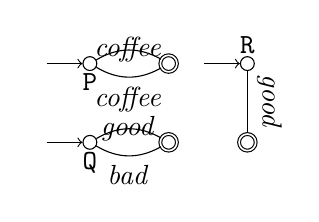
\begin{tikzpicture}
    \tikzstyle{every state}=[
        draw,
        shape=circle,
        inner sep=1pt,
        minimum size=5pt,
        final/.style={double,minimum size=6pt},
        initial text=] 

    [->,auto,node distance=1.5cm]
    \renewcommand{\a}[1]{\textit{#1}}
    \node[state,initial] (a0) {}; 
    \node[state, final, right of=a0] (a1) {};
    \node[state,initial,below of=a0] (b0) {}; 
    \node[state, final, right of=b0] (b1) {};
    \node[state,initial,right of=a1] (c0) {}; 
    \node[state, final, below of=c0] (c1) {};
    \path (a0) node[below]{\ttfamily P} (a0) edge[bend left] node{\a{coffee}} (a1)
                                                edge[bend right] node[below]{\a{coffee}} (a1)
            (b0) node[below]{\ttfamily Q} (b0) edge[bend left] node{\a{good}} (b1)
                                                edge[bend right] node[below]{\a{bad}} (b1)
            (c0) node[above]{\ttfamily R} (c0) edge node[above,rotate=-90]{\a{good}} (c1);
\end{tikzpicture}
\end{document}